\chapter{Introduction}


\vspace{2mm}

\section{Motivation}
\textbf{Author: Sztavinovszki}
In almost every robotics application nowadays you need some kind of communication. Wether it is a robot communicating
its data to a home-base, or two robots sharing data with one another. Over the past years communication has drastically
improved with new protocols and technology, such as Bluetooth Low energy.

\section{Goal}
\textbf{Author: Sztavinovszki}

\section{History}
\textbf{Author: Dragosits}
\subsection{Networks}
The history of communication and coordination between seperate systems is long and extensive. Nowadays it is an essential 
function of almost every technological device. In the field of computing it started in the late 1950s with SAGE (Semi-Automatic Ground Enviornment),
which was a network of computers and networking technology created by the United States of America military, 
and it allowed the transfer of radar data nation-wide.\footcite[][89]{A_New_History_of_Modern_Computing}
The next major step forward was the beginning of ARPANET in 1969, which served as a connection between multiple north american 
universities, and laid the groundwork for the modern internet.\footcite[][25]{How_the_web_was_born}
In more recent times the Internet of Things is commonplace, and is used for the interchange of terabytes of data each day. 
But there are also many smaller private networks used either for simple processes or sensitive data, that shouldn't be 
accesible by a theoretical viewer outside the trusted circle. 

\subsection{Protocols}
Nowadays there are a wide variety of protocols for the transfer of data across a network. However the protocol TCP has cemented 
itself as the most popular of the Transport layer protocols, due to its use in the internet. TCP/IP was first described in
RFC 675\footcite{rfc_675}, where the authors laid the groundwork for modern network communication. Another protocol that uses IP
is UDP. Developed by David Patrick Reed in 1980 it and TCP are some of the most commonly used methods of transfering data across
the internet and similar networks. Both of these alongside IP are the foundation of the Internet Protocol Suite.   

\subsection{Bluetooth}
The communication between multiple mobile and fixed devices over short distances and the formation of personal area networks (PANs)
has historically been cumbersome. Bluetooth is a technology created in order to solve this. The original idea was concieved in 1989
at Ericsson Mobile in oder to create wireless headsets. Development began later in 1994 and in 1997 the company was approched by IBM
for a collaberation on the IBM Thinkpad. This technology was then implemented on both the Thinkpad notebook and an Ericsson mobile phone.
Afterwards the first device with Bluetooth functionality was revealed to be a wireless headset in 1999.

\section{Project Management}
\textbf{Author: Sztavinovszki}

\section{Outline}
%\section{Section}
%More text. \lipsum[1] See Figure~\ref{pic:example}.

%\begin{figure}[h]
%	\centering
%	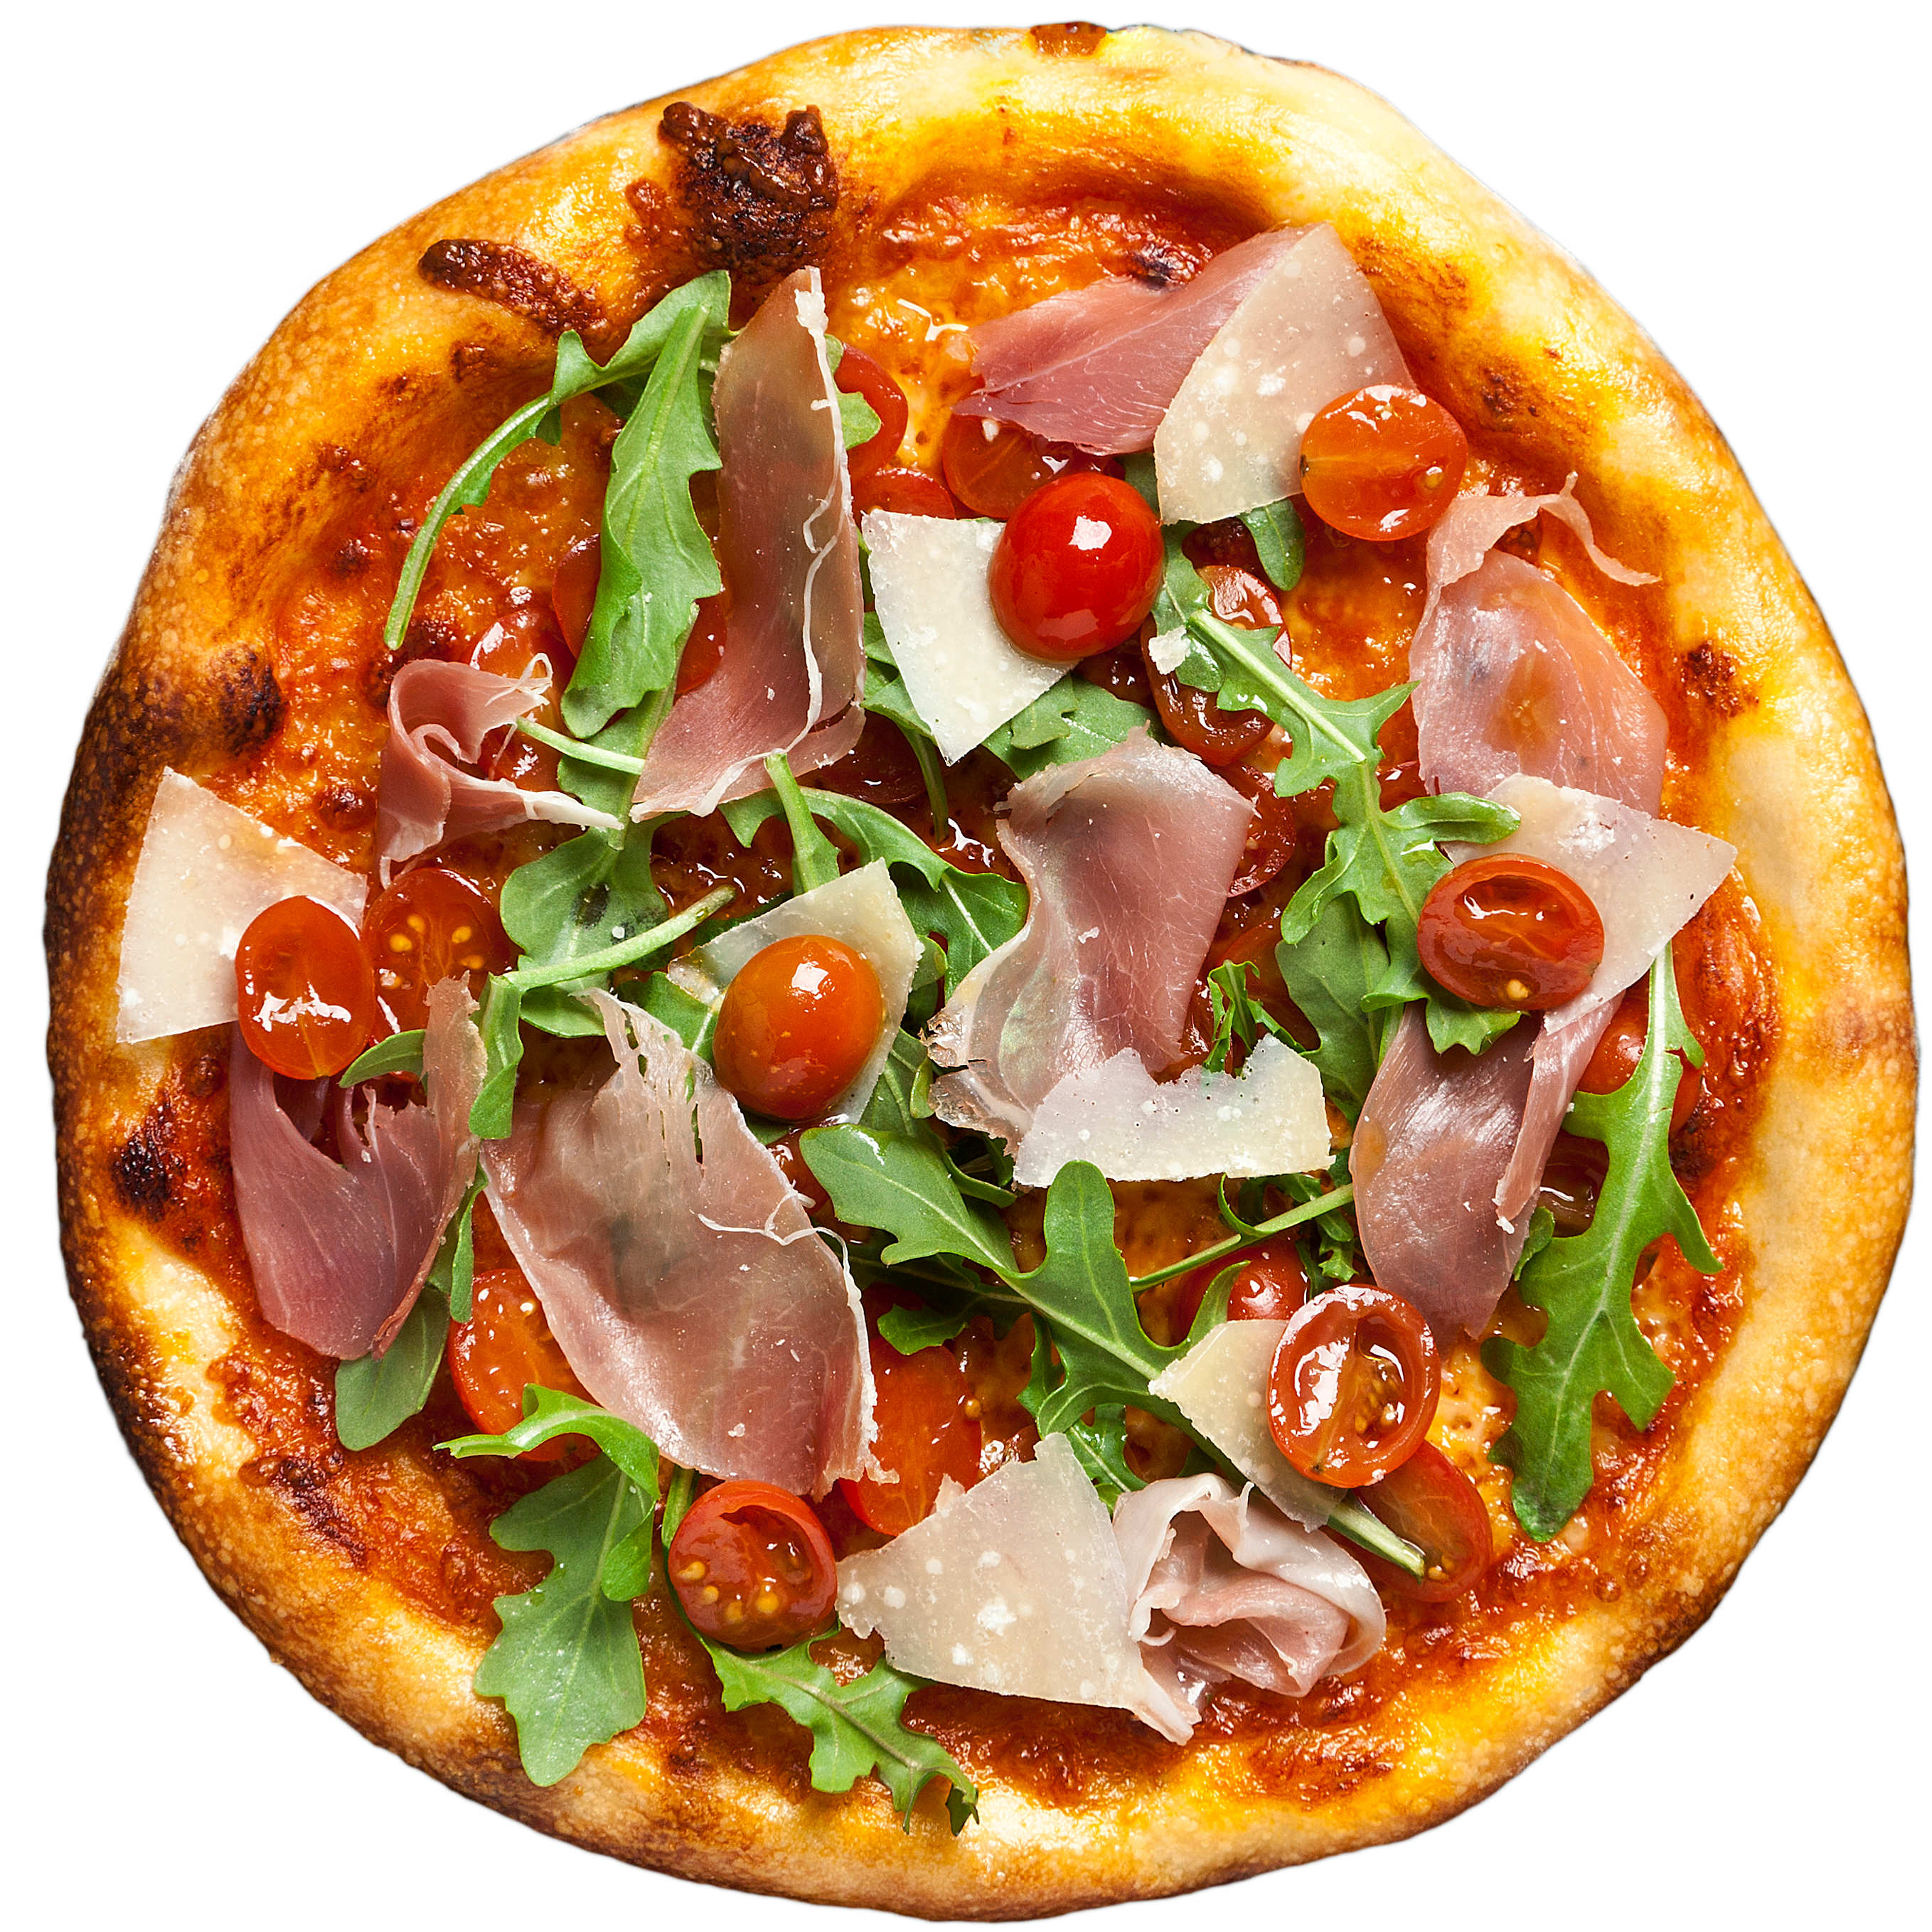
\includegraphics[width=2.5in]{img/example.png}
%	\caption{Picture description.}
%	\label{pic:example}
%\end{figure}

%\subsection{Subsection}
%\lipsum[1]

%\subsection{Subsection}
%\lipsum[1] See Table~\ref{tab:example}.

%\begin{center}
%	\begin{tabular}{| l | l | l |}
%		\hline
%		\bfseries Header 1 & \bfseries Header 2 & \bfseries Header 2 \\
%		\hline
%		Text & text & text \\
%		\hline
%		Text & text & text  \\
%		\hline
%		Text & text & text  \\
%		\hline
%	\end{tabular}
%	\label{tab:example}
%\end{center}

%\lipsum[1] Some references can be found at \footcite{robo4you} or at \footcite{Hope_Learning_TensorFlow}.
%

\filbreak
